\begin{frame}{Gambling Experiment}
\textbf{Goal}: Study the effect of stress on risky decision making \par
\textbf{Stress measures}:
	\begin{description}
		\item[BP] Blood Pressure
		\item[HR] Heart Rate
		\item[GSR] Galvanic skin response
		\item[STAI] State train anxiety inventory
		\item[CRT] Cortisol
	\end{description}
\textbf{Problem}:
	\begin{enumerate}
		\item How do we know our stress manipulation works?
		\item How to we quantify stress?
	\end{enumerate}
\end{frame}

\begin{frame}
	\begin{center}
        		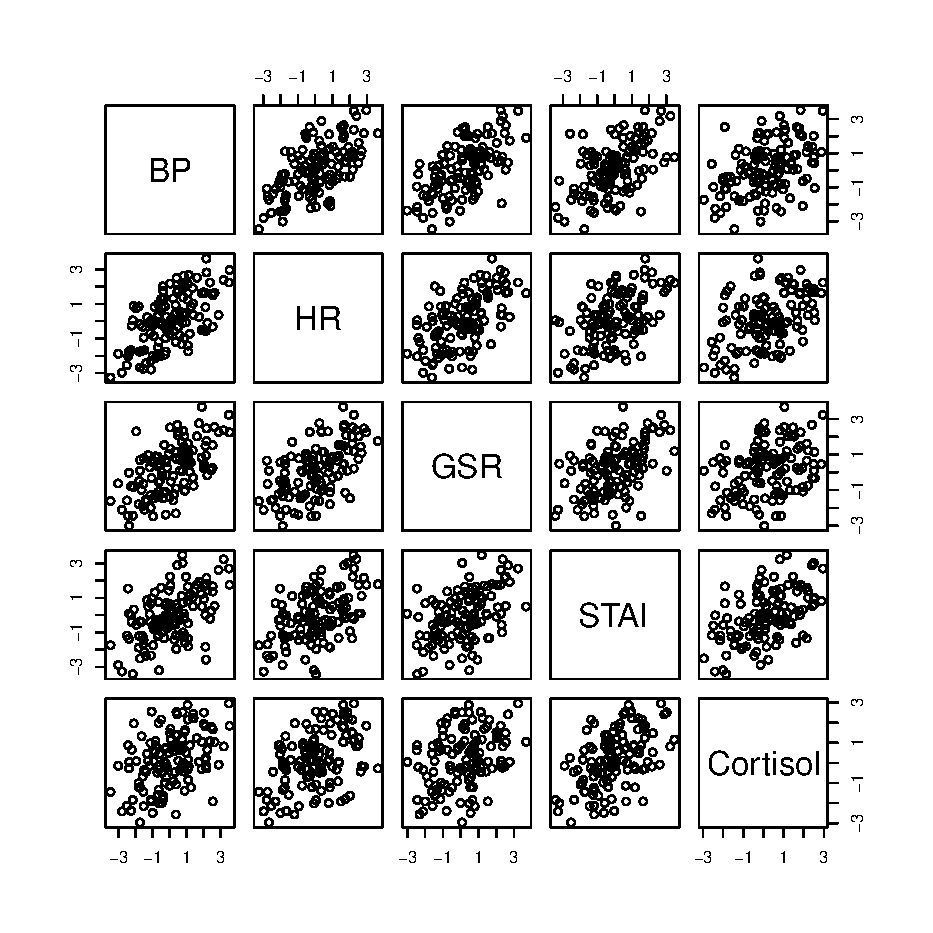
\includegraphics[scale=.5, center]{figures/stress_pairs.eps}
    	\end{center}
\end{frame}

\begin{frame}{Intuition}
	\begin{minipage}{0.47\textwidth}
    		\begin{center}
        		\includegraphics[scale=.25, center]{figures/stress_comp1.png}
    		\end{center}
	\end{minipage}
	\begin{minipage}{0.5\textwidth}
    		\begin{center}
        		\includegraphics[scale=.25, center]{figures/stress_comp2.png}
    		\end{center}
	\end{minipage}
\end{frame}